\titre{Pourquoi des applications réparties ?} 
\begin{itemize}
	\item Partage et mise en commun des ressources
	\item Domaines nouveaux d'applications
	\item Intégration d'objets du monde réel : informatique pervasive
	\item Convergence forte entre informatique et télécommunications
	\item Parallélisme pour la puissance de traitements (grid computing)
\end{itemize}

\titre{Définition :} Qu'est-ce qui caractérise une application répartie ?
\begin{itemize}
	\item Le temps
	\item La distance
	\item Multimachine
	\item Persistance des données
\end{itemize}

\titre{Exercice 1} Structure d'un chat \\
	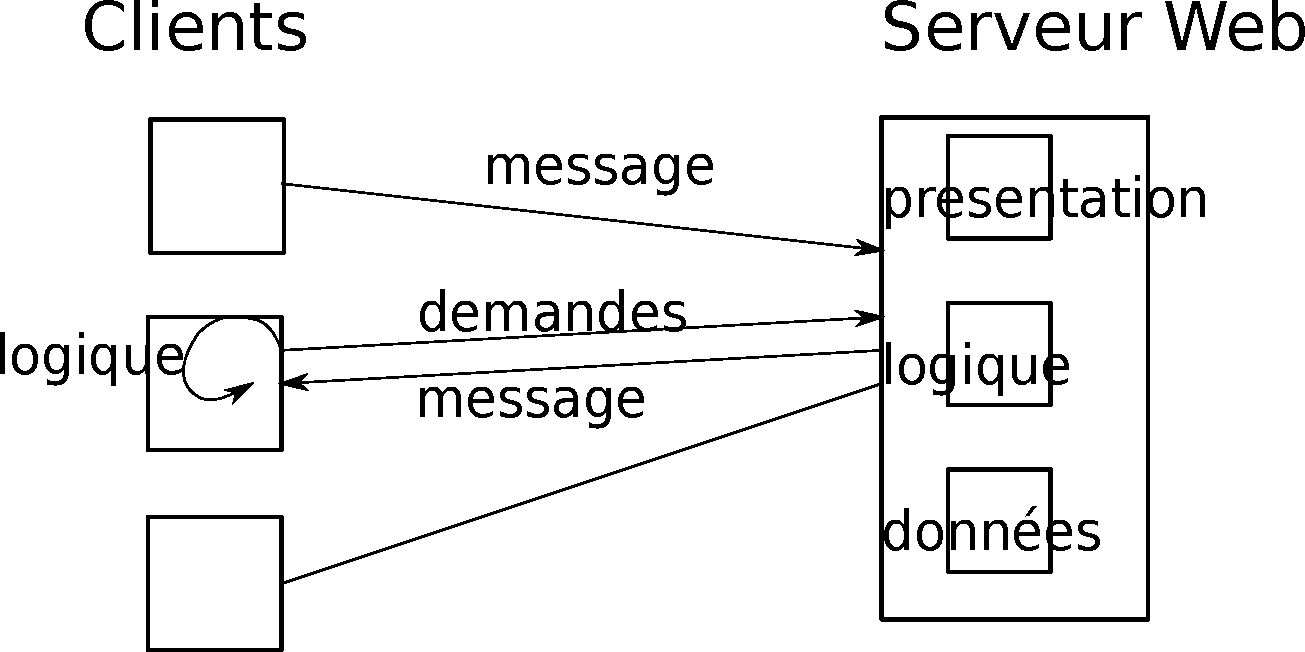
\includegraphics[width=150px]{Images/01_exo1a.pdf} \\
	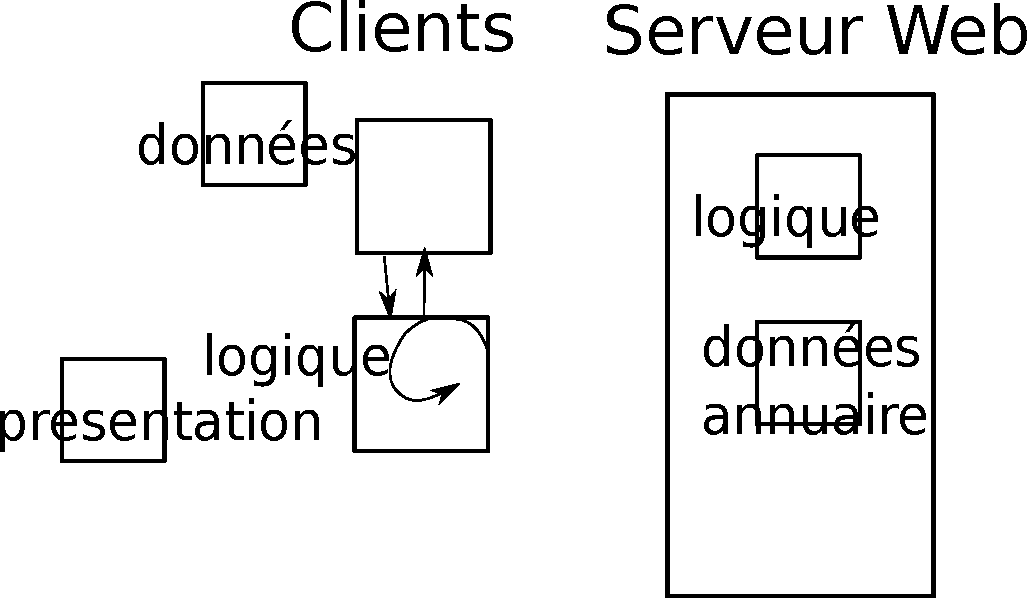
\includegraphics[width=150px]{Images/01_exo1b.pdf} \\

\titre{Exercice 2} Mail \\
	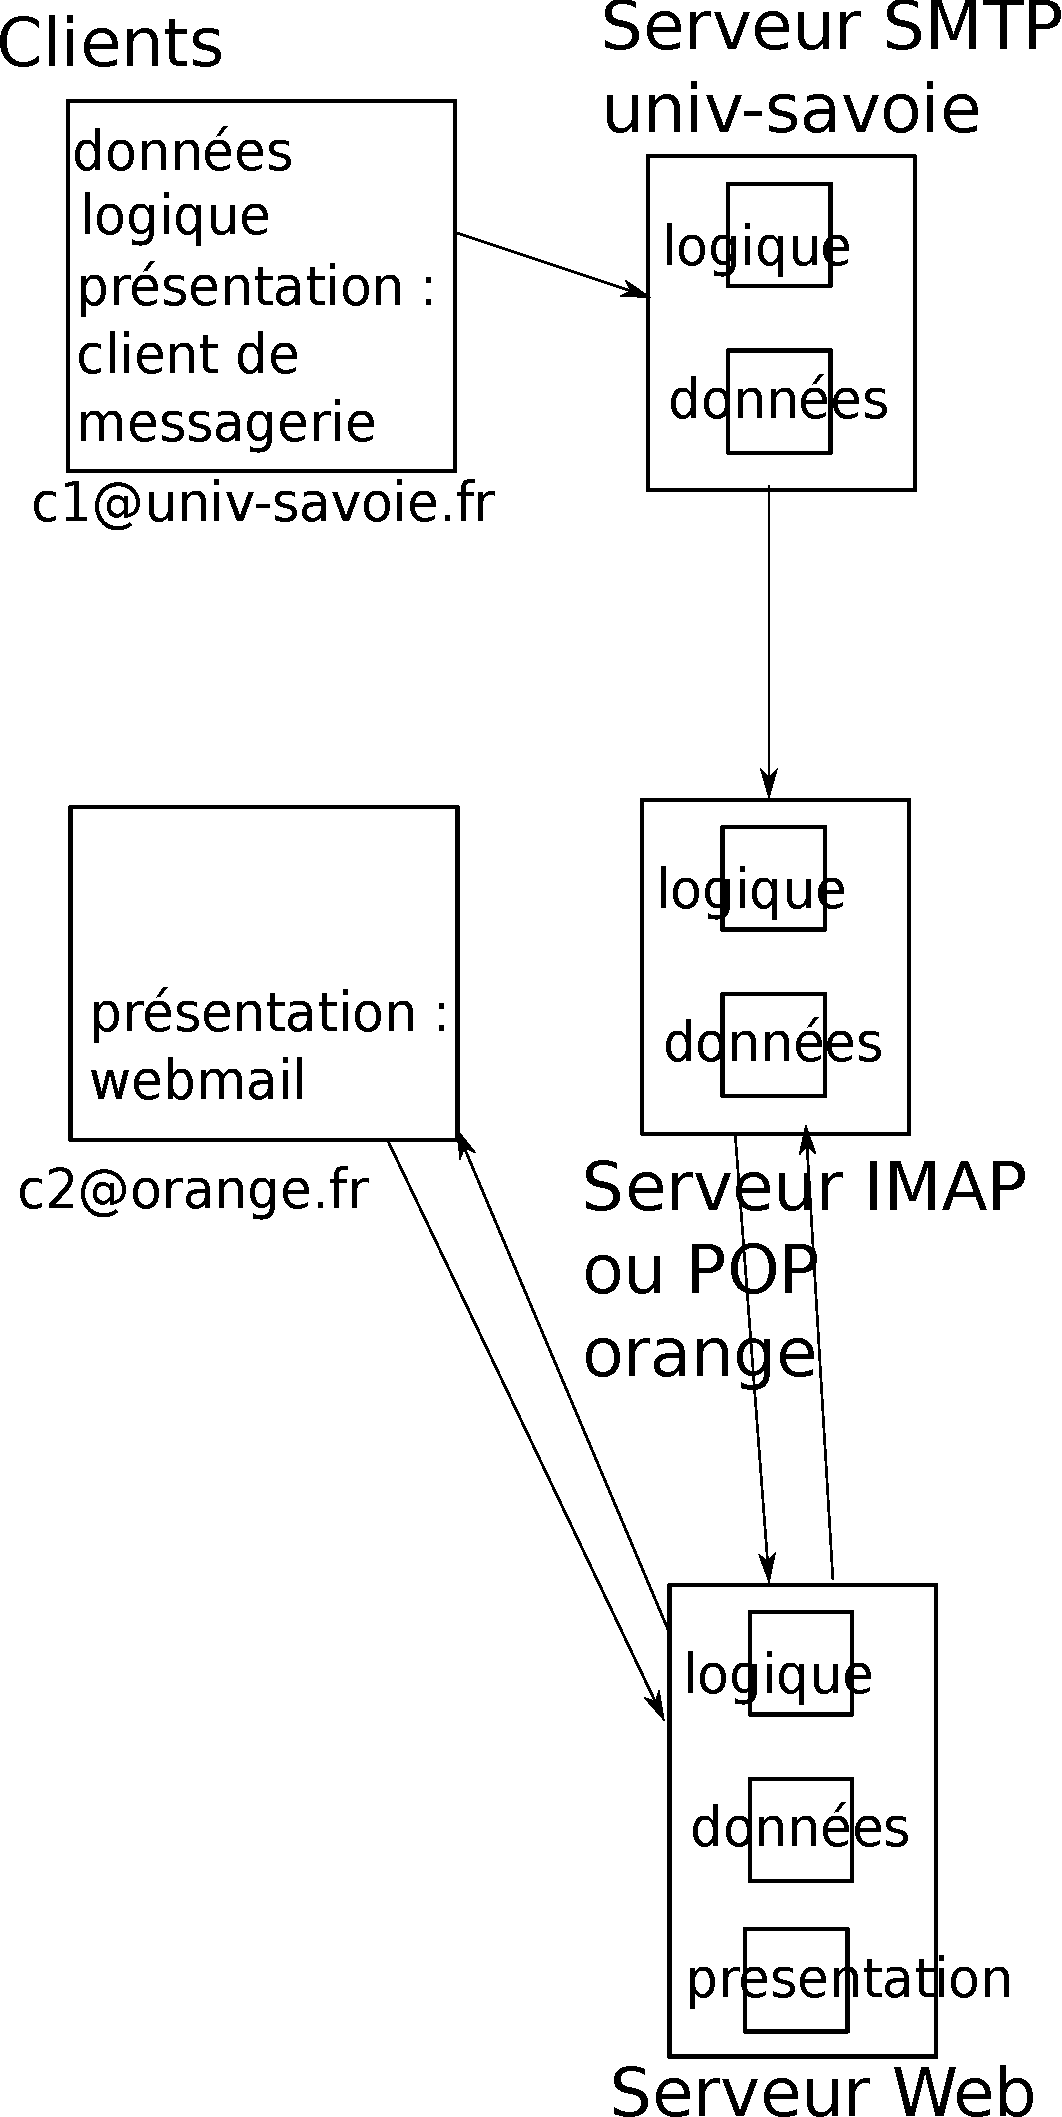
\includegraphics[width=100px]{Images/02_exo2.pdf} \\

\titre{Exercice 3} Service d'échanges de fichiers \\

\titre{Ce que doit offrir un système réparti}
\begin{itemize}
	\item Transparence à la localisation
	\item Transparence d'accès
	\item Transparence à l'hétérogénéité
	\item Transparence aux pannes
	\item Transparence à l'extension des ressources
\end{itemize}

\titre{Tendance générale :} Intégration de haut niveau
